\section{Faster Regional-CNN}
\subsection{Stage 1}
CNN Backbone extracts a feature map. Each pixel of the feature map becomes an anchor point. There are 9 different anchor boxes (feature map* 9). Each \textbf{anchor box} is compared with the ground truth box. If the score \textgreater{} 0.7, it is a positive box. The highest score wins. To compare IoU is used.
For each anchor box, we derive a corresponding ground truth box and filter them based on positive boxes (red). Since each ground truth box has a category, we can apply the same principle to obtain positive categories. Next, we calculate the offsets of the anchor boxes to the ground truth boxes (Fig \ref{fig:faster_r_cnn_stage_1}).

Anchor Box + Offset = Region Proposal

\begin{figure}[ht]
  \centering
  \subfloat[IoU]{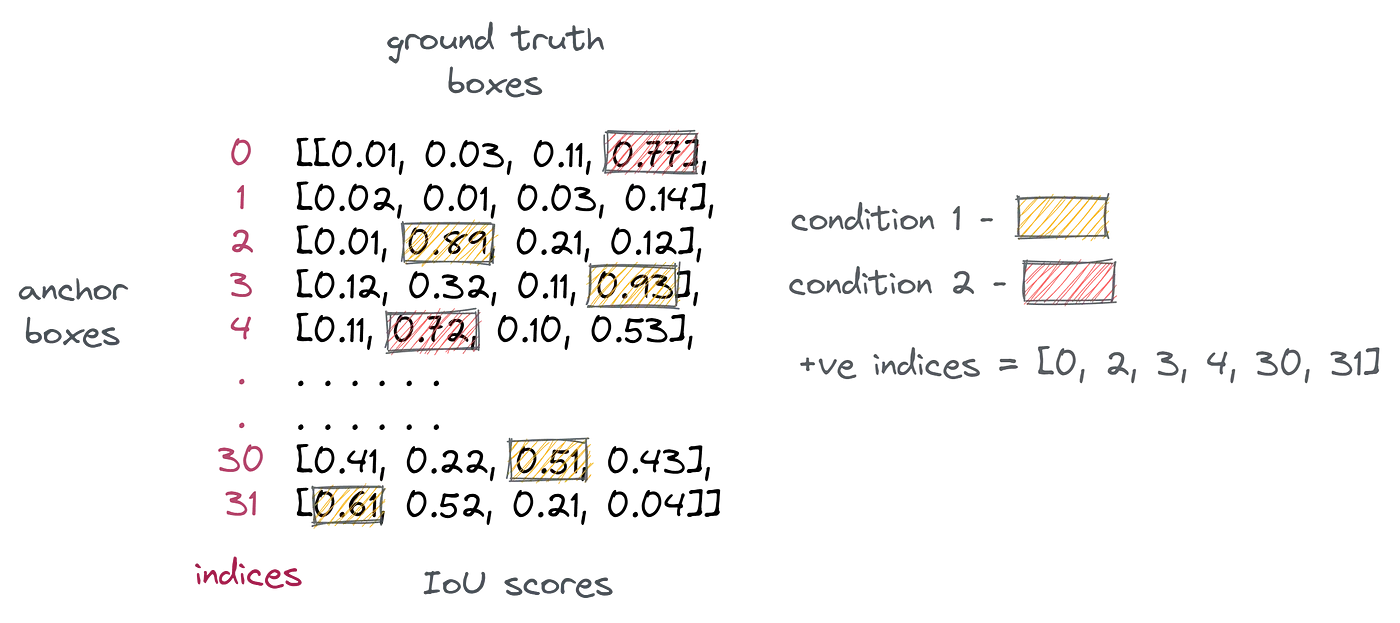
\includegraphics[width=0.5\textwidth]{images/faster_r_cnn/positive_anchor.png}\label{fig:f1}}
  \hfill
  \subfloat[Filter Positive Groundtruth]{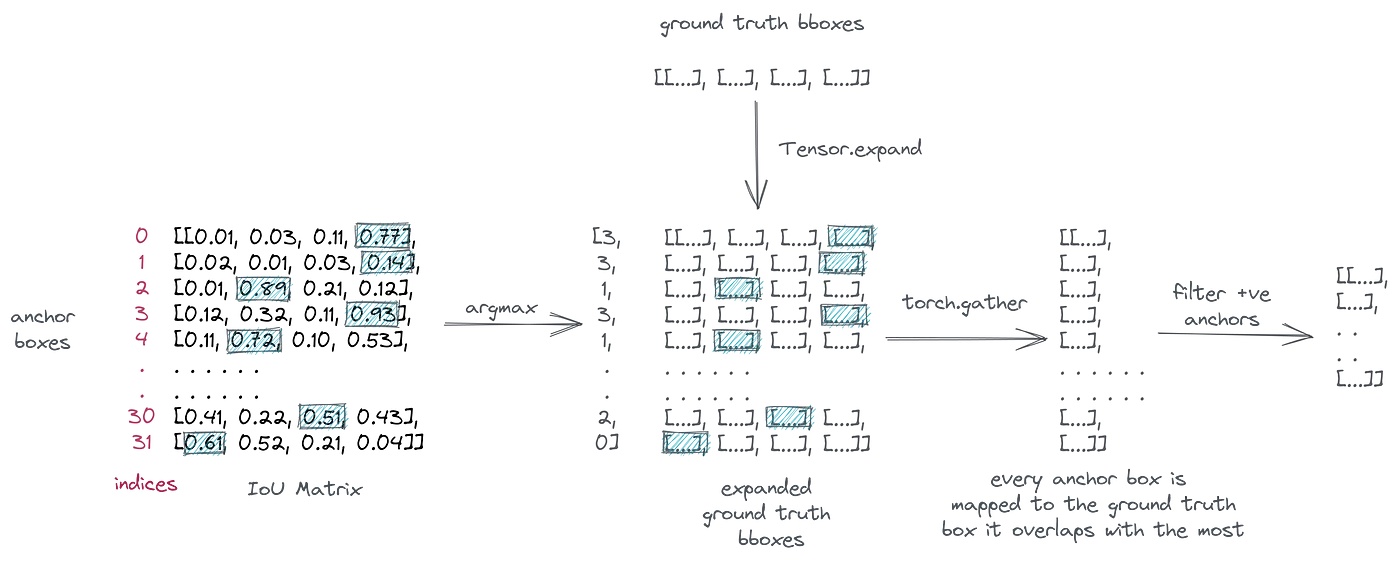
\includegraphics[width=0.5\textwidth]{images/faster_r_cnn/filter_positive_gt.png}\label{fig:f2}}
  \caption{Stage 1}
  \label{fig:faster_r_cnn_stage_1}
\end{figure}

\subsection{Stage 2}

The region proposals are divided into a fixed number of regions and then max pooling is applied. This ensures that the regions have the same dimension (ROI). Cross Entropy Loss learns the categories. Regression learns the offsets (Fig \ref{fig:faster_r_cnn_structure}).

\begin{figure}[H]
  \centering
  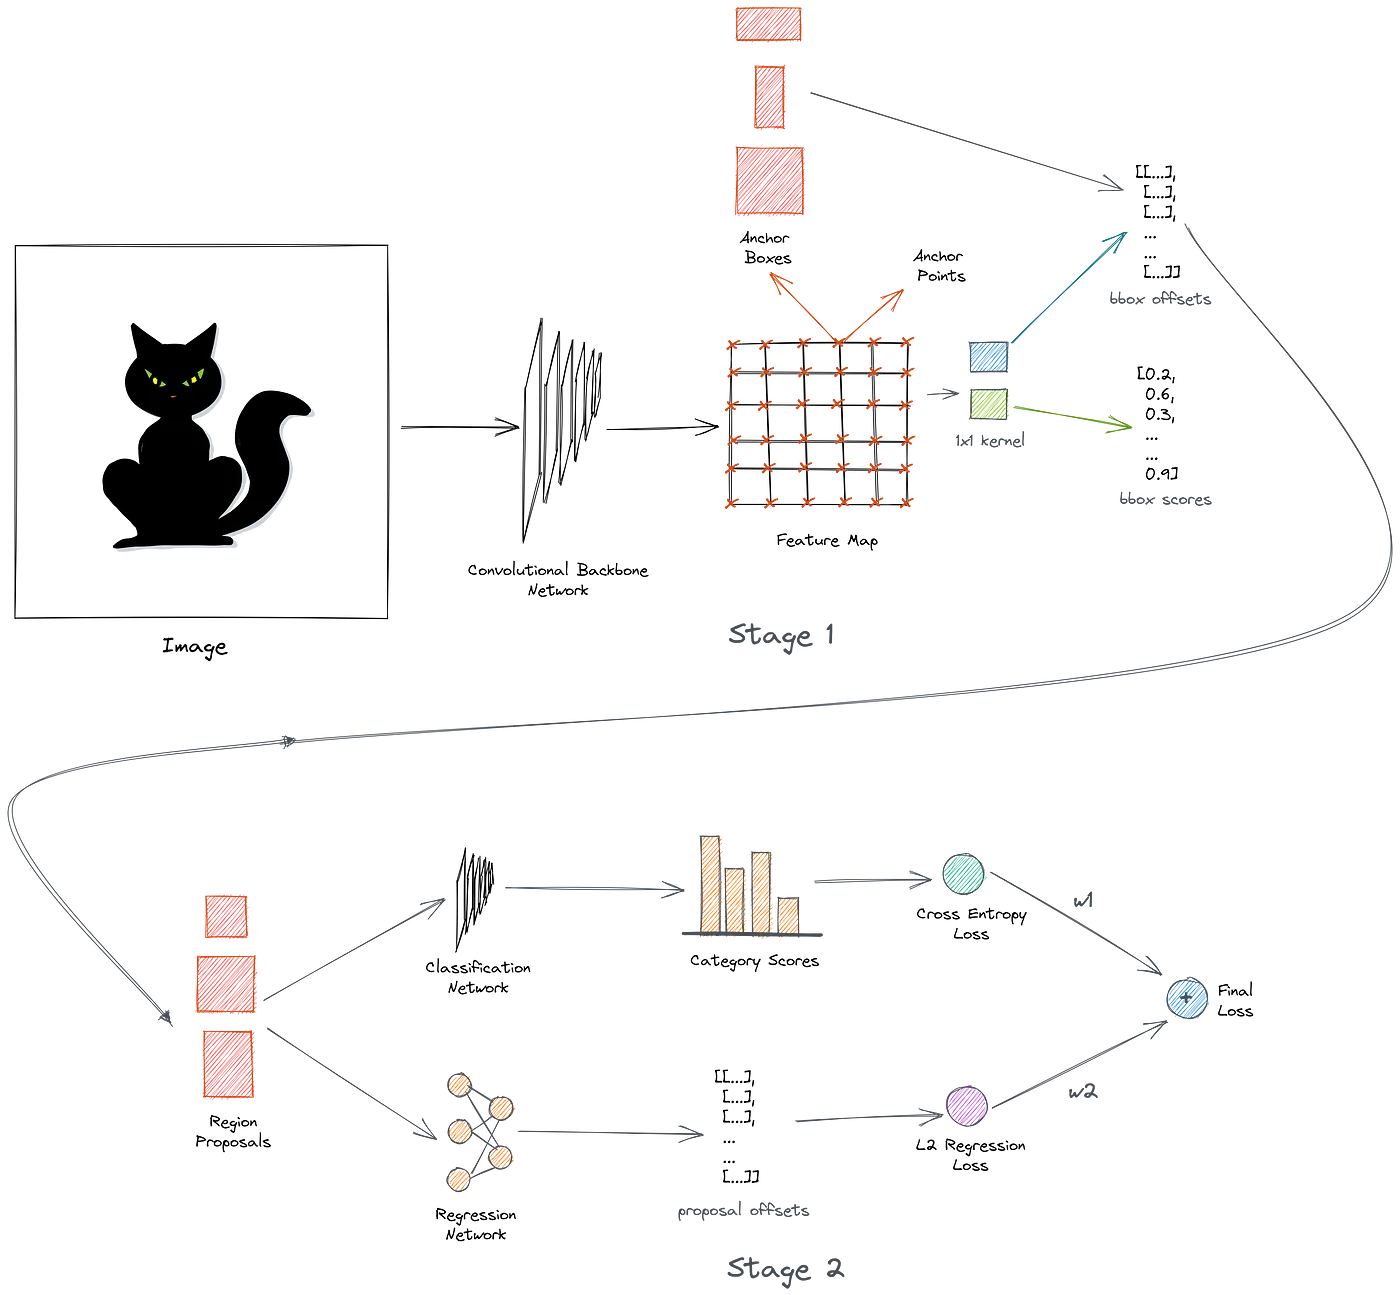
\includegraphics[width=0.8\textwidth]{images/faster_r_cnn/structure.png}
  \caption{Faster RCNN}
  \label{fig:faster_r_cnn_structure}
\end{figure}

\subsection{Sources}

\begin{enumerate}
  \item \href{https://towardsdatascience.com/understanding-and-implementing-faster-r-cnn-a-step-by-step-guide-11acfff216b0}{TowardsDataScience}
\end{enumerate}
